\fancyhead{}
\fancyfoot{}
\cfoot{\thepage}

\lhead{Anexos}
%\rhead{\today}
%\rfoot{\thepage}

\chapter{Anexos}

\begin{figure}[H]
  \begin{center}
    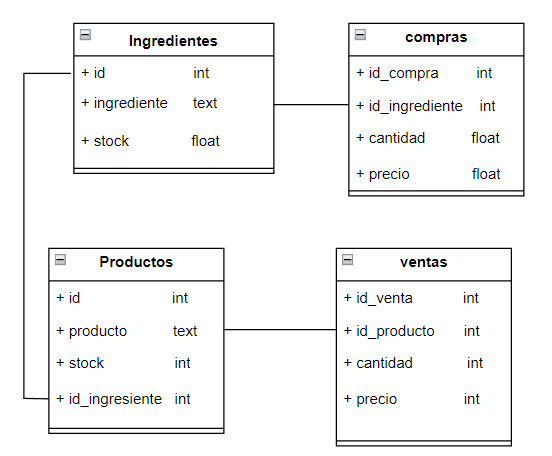
\includegraphics[scale=0.70]{./diagrama de clases.png}
    \caption{Diagrama de clases sistema de
    gestion de inventario.}
    \label{fig:product}
  \end{center}
\end{figure}

El diagrama de clases del sistema comprende cuatro entidades principales: Compras, Ventas, Productos e Ingredientes. La clase Ingredientes incluye atributos como id, que funciona como clave primaria, el ingrediente en sí representado por la descripción y la cantidad en stock. Por otro lado, la clase Productos cuenta con atributos como id, que sirve como clave primaria, la descripción del producto, la cantidad en stock y una relación con la clase Ingredientes a través del id\_ingrediente. De esta manera, las clases Compras y Ventas registran transacciones asociadas a estos productos e ingredientes, incluyendo detalles como el id\_compra o id\_venta, respectivamente, la cantidad y el precio. Este diseño de clases proporciona una estructura coherente para gestionar eficientemente las operaciones de compra y venta, manteniendo un control detallado sobre los productos e ingredientes disponibles en el sistema.
\begin{figure}[H]
    \begin{center}
        \begin{subfigure}{0.28\textwidth}
            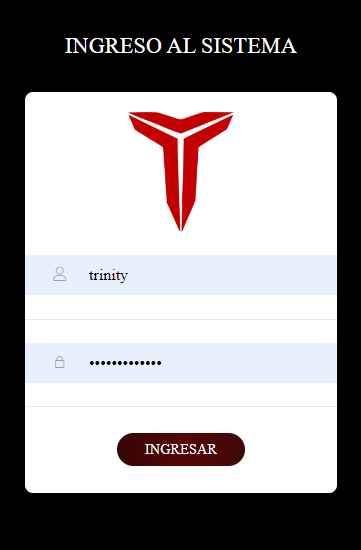
\includegraphics[width=\linewidth]{./sistema/login.png}
            \caption{Interfaz de inicio}
        \end{subfigure}
        \hspace{0.05\textwidth}
        \begin{subfigure}{0.62\textwidth}
            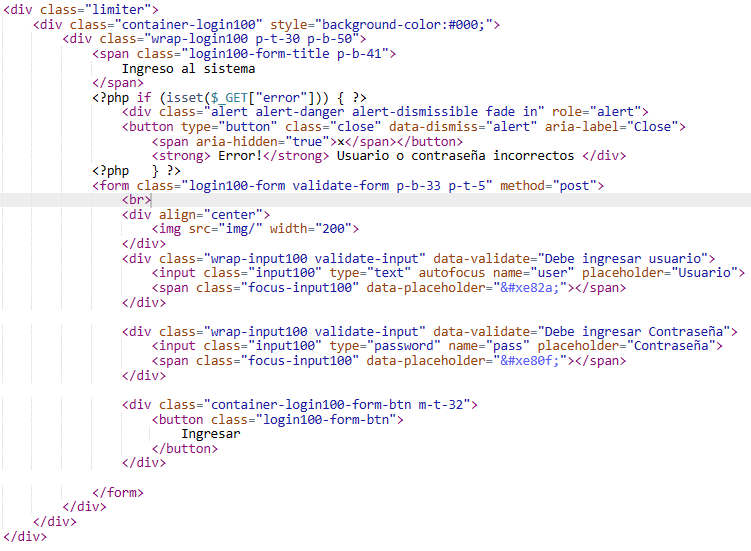
\includegraphics[width=\linewidth]{./sistema/codigo_login.png}
            \caption{Código de inicio de sesión del sistema}
        \end{subfigure}
        \caption{Login del sistema}
        \label{fig:login}
    \end{center}
\end{figure}

Este script PHP se utiliza para la autenticación de usuarios en un sistema web, empleando PHP y MySQL para gestionar la base de datos de usuarios. También se hace uso de tecnologías web como HTML, CSS. para el diseño del formulario de inicio de sesión. El script verifica las credenciales ingresadas por el usuario y, en caso de ser correctas, inicia una sesión y redirige al usuario a una página específica en función de su nivel de acceso. Si las credenciales son incorrectas, se muestra un mensaje de error.


\begin{figure}[H]
    \begin{center}
      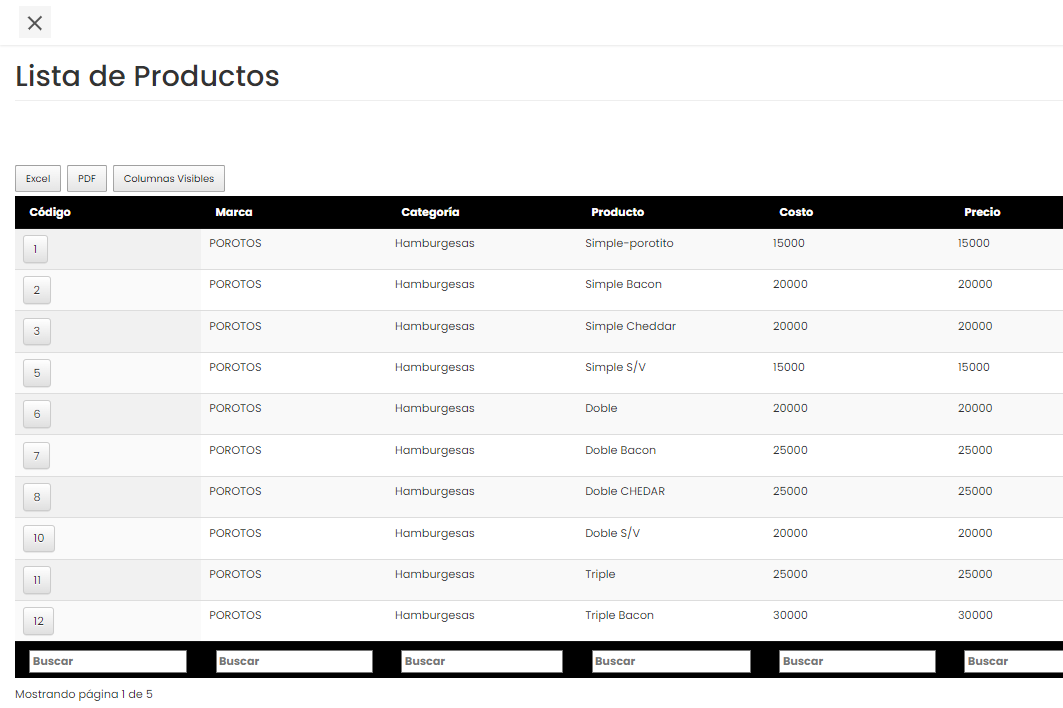
\includegraphics[scale=0.45]{./sistema/lista productos.png}
      \caption{Interfaz productos}
      \label{fig:product}
    \end{center}
  \end{figure}

  \begin{figure}[H]
    \begin{center}
      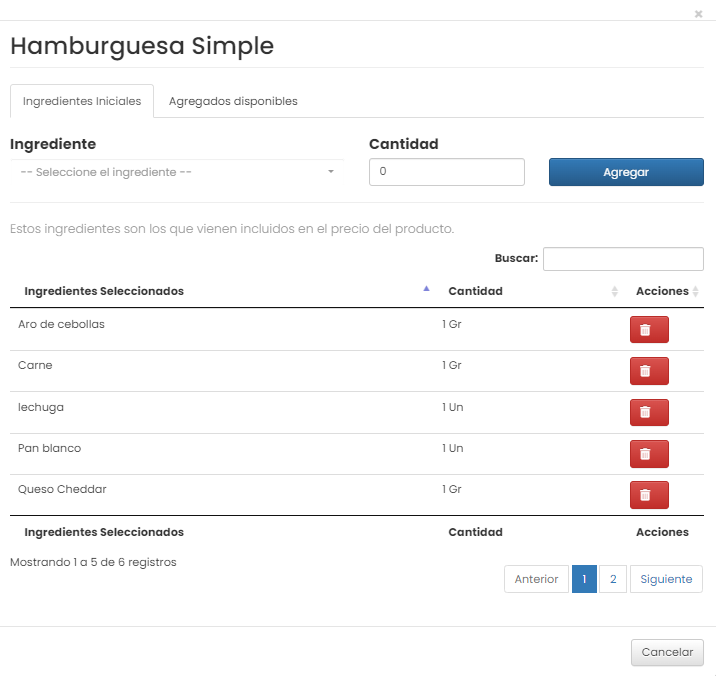
\includegraphics[scale=0.50]{./sistema/ingrediente_de_producto.png}
      \caption{Interfaz de carga de ingredientes}
      \label{fig:product}
    \end{center}
  \end{figure}

  \begin{figure}[H]
    \begin{center}
      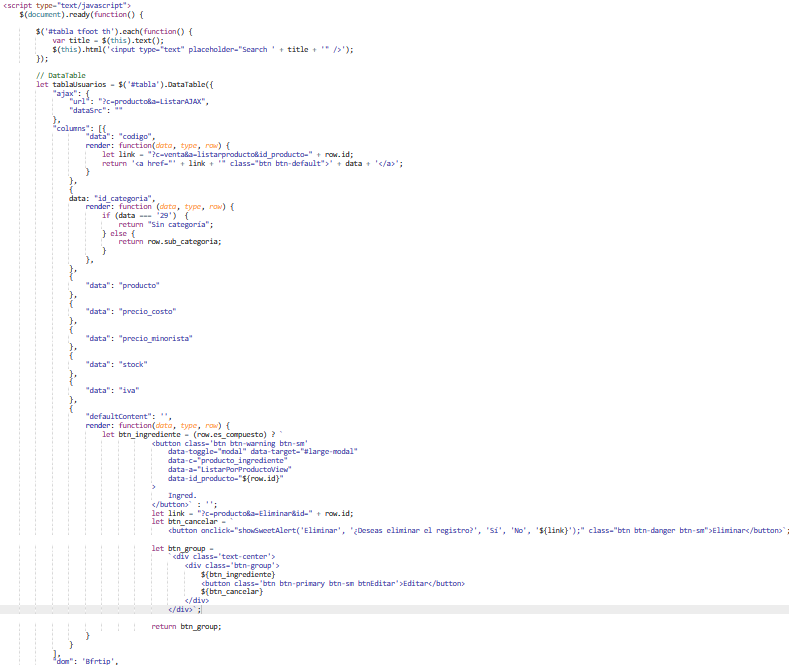
\includegraphics[scale=0.90]{./sistema/producto_codigo.png}
      \caption{Codigo carga de productos e ingresientes}
      \label{fig:product}
    \end{center}
  \end{figure}

El código proporcionado es una combinación de HTML, PHP y JavaScript que se utiliza para crear una página web que muestra una lista de productos. Emplea HTML para estructurar la página, PHP para interactuar con una base de datos y recuperar datos de productos, y JavaScript, incluyendo la biblioteca DataTables, para agregar funcionalidades interactivas a la tabla de productos. La página permite buscar, editar y eliminar productos, y utiliza solicitudes AJAX para comunicarse con el servidor y obtener información sobre los productos. En conjunto, estas tecnologías y herramientas se utilizan para construir una interfaz web dinámica y amigable para la gestión de productos \cite{mohedano2012iniciacion}.

\begin{figure}[H]
    \begin{center}
      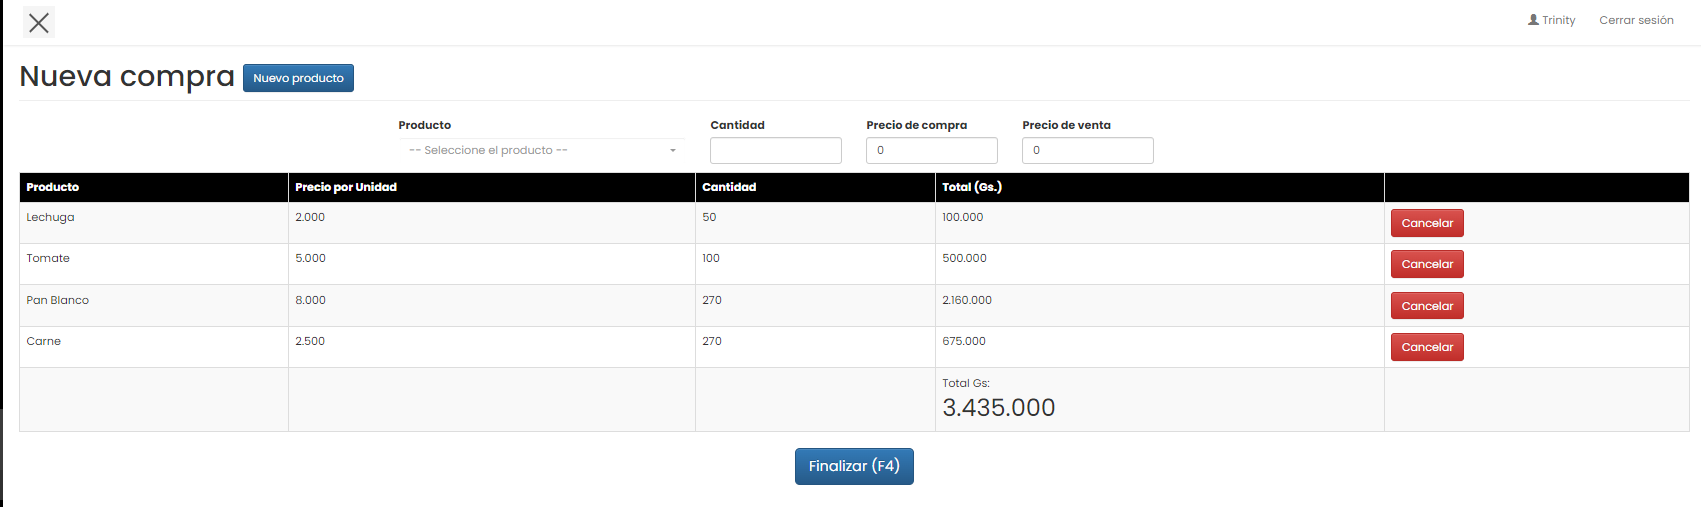
\includegraphics[scale=0.30]{./sistema/compras.png}
      \caption{Interfaz de compras }
      \label{fig:product}
    \end{center}
  \end{figure}
  \begin{figure}[H]
    \begin{center}
      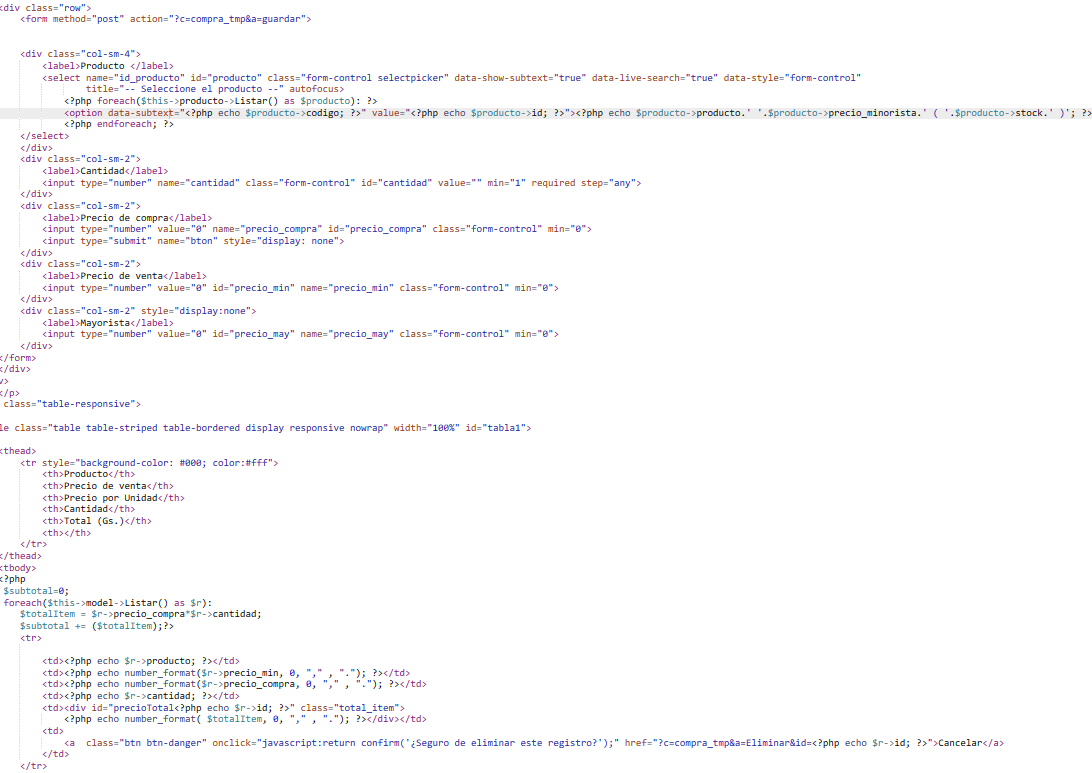
\includegraphics[scale=0.55]{./sistema/codigo_compra.png}
      \caption{Codigo carga de compras }
      \label{fig:product}
    \end{center}
  \end{figure}
  Este código HTML muestra un formulario que permite a los usuarios ingresar detalles de productos, como seleccionar un producto, definir la cantidad, el precio de compra y el precio de venta.

  \begin{figure}[H]
    \begin{center}
      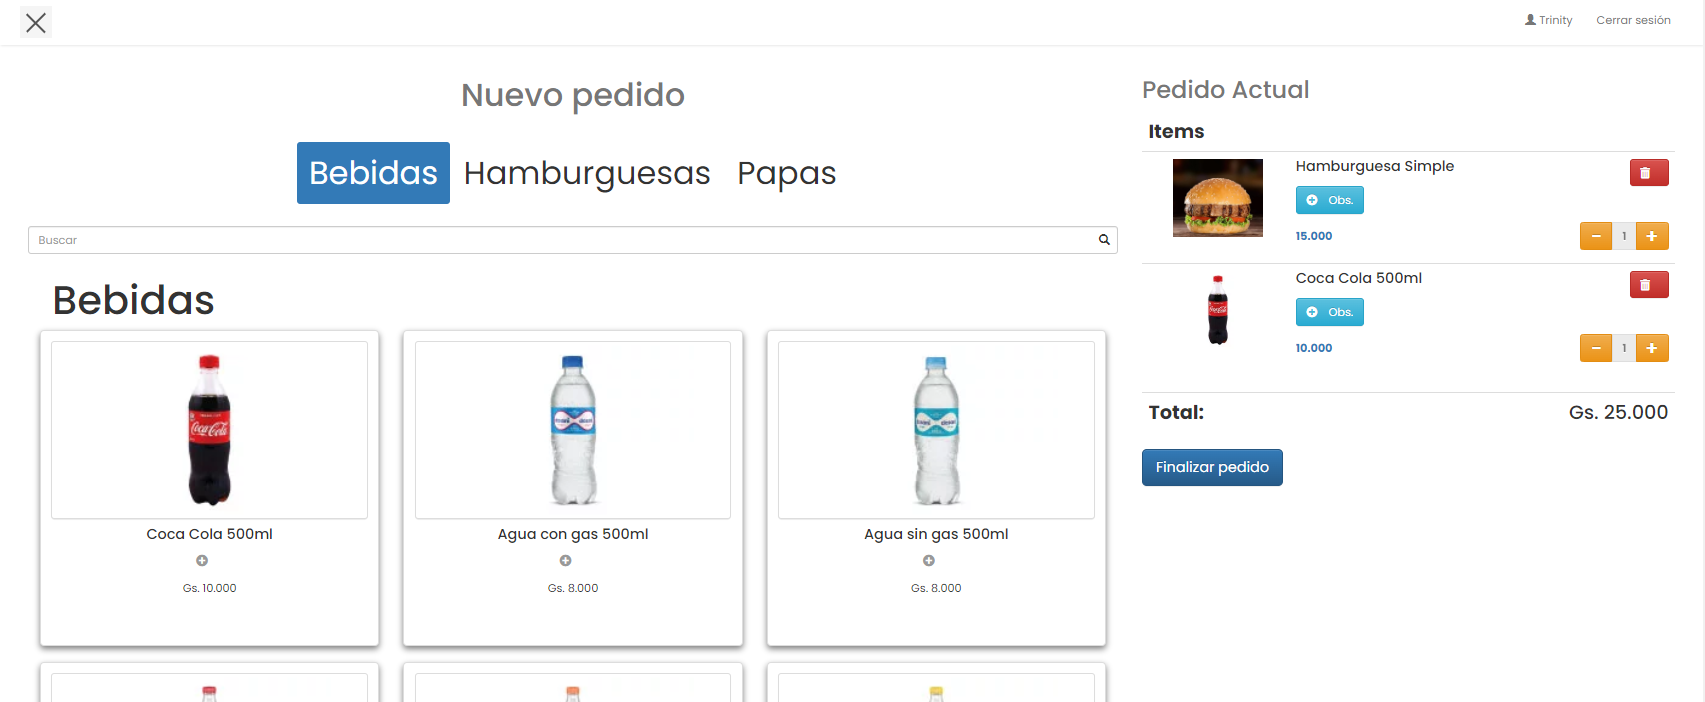
\includegraphics[scale=0.25]{./sistema/nueva_venta.png}
      \caption{Interfaz de ventas}
      \label{fig:product}
    \end{center}
  \end{figure}
  \begin{figure}[H]
    \begin{center}
      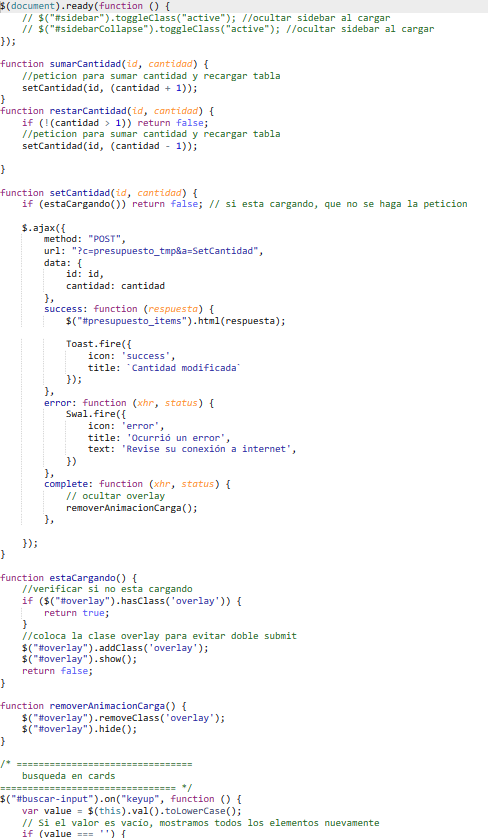
\includegraphics[scale=0.65]{./sistema/codigo_venta.png}
      \caption{Codigo carga de ventas}
      \label{fig:product}
    \end{center}
  \end{figure}

  \begin{figure}[H]
    \begin{center}
      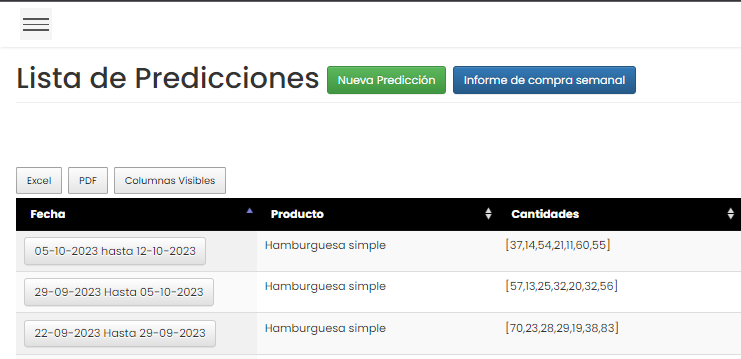
\includegraphics[scale=0.65]{./sistema/lista_predicciones.png}
      \caption{Interfaz de lista de predicciones hechas}
      \label{fig:product}
    \end{center}
  \end{figure}

  \begin{figure}[H]
    \begin{center}
      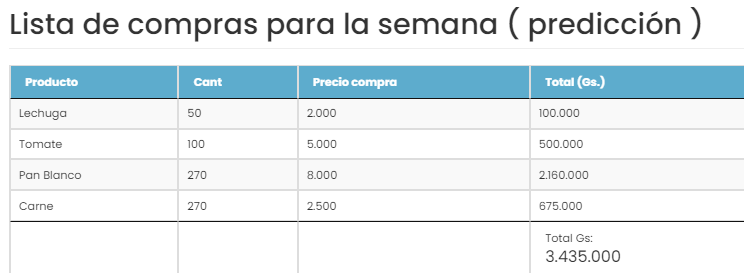
\includegraphics[scale=0.65]{./sistema/Informe de compra prediccion.png}
      \caption{Informe de predicción de ingredientes a comprar }
      \label{fig:product}
    \end{center}
  \end{figure}


  \begin{figure}[H]
    \begin{center}
      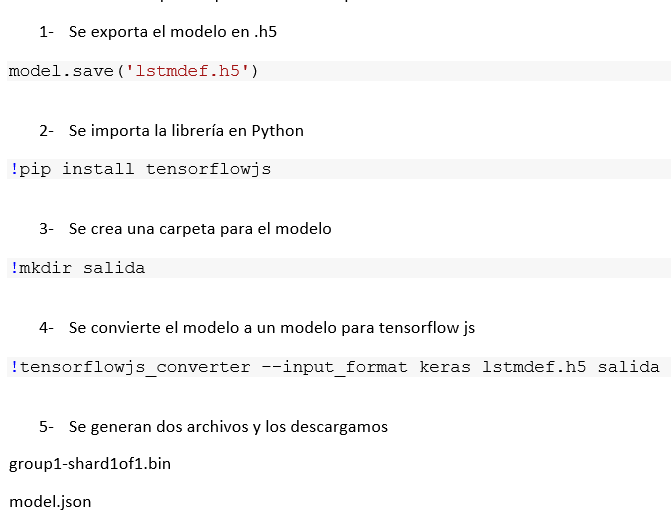
\includegraphics[scale=0.90]{./sistema/primeraparte.png}
      \caption{Expotación de Python}
      \label{fig:python}
    \end{center}
  \end{figure}

  \begin{figure}[H]
    \begin{center}
      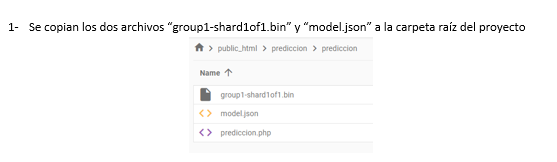
\includegraphics[scale=0.90]{./sistema/segundaparte.png}
      \caption{Importación a javascript}
      \label{fig:python}
    \end{center}
  \end{figure}

  \begin{figure}[H]
    \begin{center}
      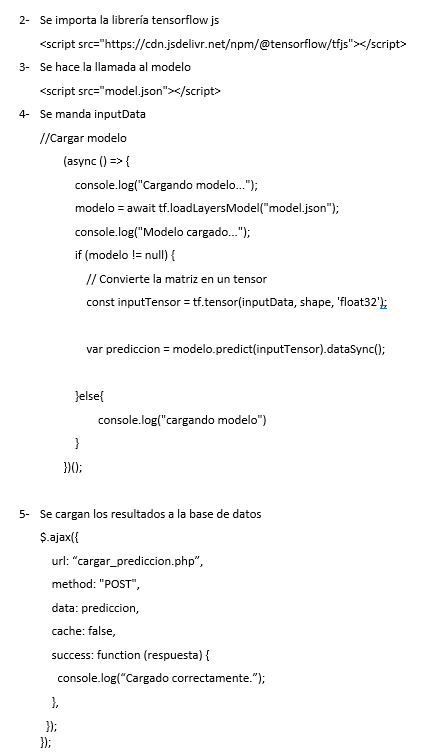
\includegraphics[scale=0.90]{./sistema/terceraparte.png}
      \caption{Importación a javascript}
      \label{fig:python}
    \end{center}
  \end{figure}


